\documentclass{article}

\usepackage{fancyhdr}
\usepackage{ragged2e}
\usepackage{graphicx}
\usepackage{caption}
\usepackage{geometry}
\usepackage{amsmath}
\usepackage{rotating}

\usepackage{listings}
\usepackage{color}

\definecolor{dkgreen}{rgb}{0,0.6,0}
\definecolor{gray}{rgb}{0.5,0.5,0.5}
\definecolor{mauve}{rgb}{0.58,0,0.82}

\lstset{frame=tb,
  language=Java,
  aboveskip=3mm,
  belowskip=3mm,
  showstringspaces=false,
  columns=flexible,
  basicstyle={\small\ttfamily},
  numbers=none,
  numberstyle=\tiny\color{gray},
  keywordstyle=\color{blue},
  commentstyle=\color{dkgreen},
  stringstyle=\color{mauve},
  breaklines=true,
  breakatwhitespace=true,
  tabsize=4
}

\setcounter{secnumdepth}{1}

\usepackage{chngcntr}
\counterwithin{figure}{section}

\renewcommand*{\thepage}{C\arabic{page}}

\pagestyle{fancy}
\lhead{ACME Robotics}
\chead{\#8367}
\rhead{\ifcontents Contents \else Week \thesection \fi}

\newif\ifcontents
\contentstrue

\makeatletter
\renewcommand{\@seccntformat}[1]{}
\makeatother

\begin{document}\contentsfalse


\subsection{Continue Developing The Team Marker}
%! Creating a releasing mechanism for the team marker. 
Shawn and Ben hadn't quite finished the anvil when they realized that the marker had no deployment mechanism and it looked super bad. They then decided to go with just a cube with a loop that could be dropped by a servo over the side. Shawn was tasked with making the block and he made it out of acrylic. Then Ben used basic Tetrix to make a servo mechanism that would unhook the cube and make it fall. Ben built the mechanism and found that a lot of servos didn't work.

\begin{figure}
    \centering
    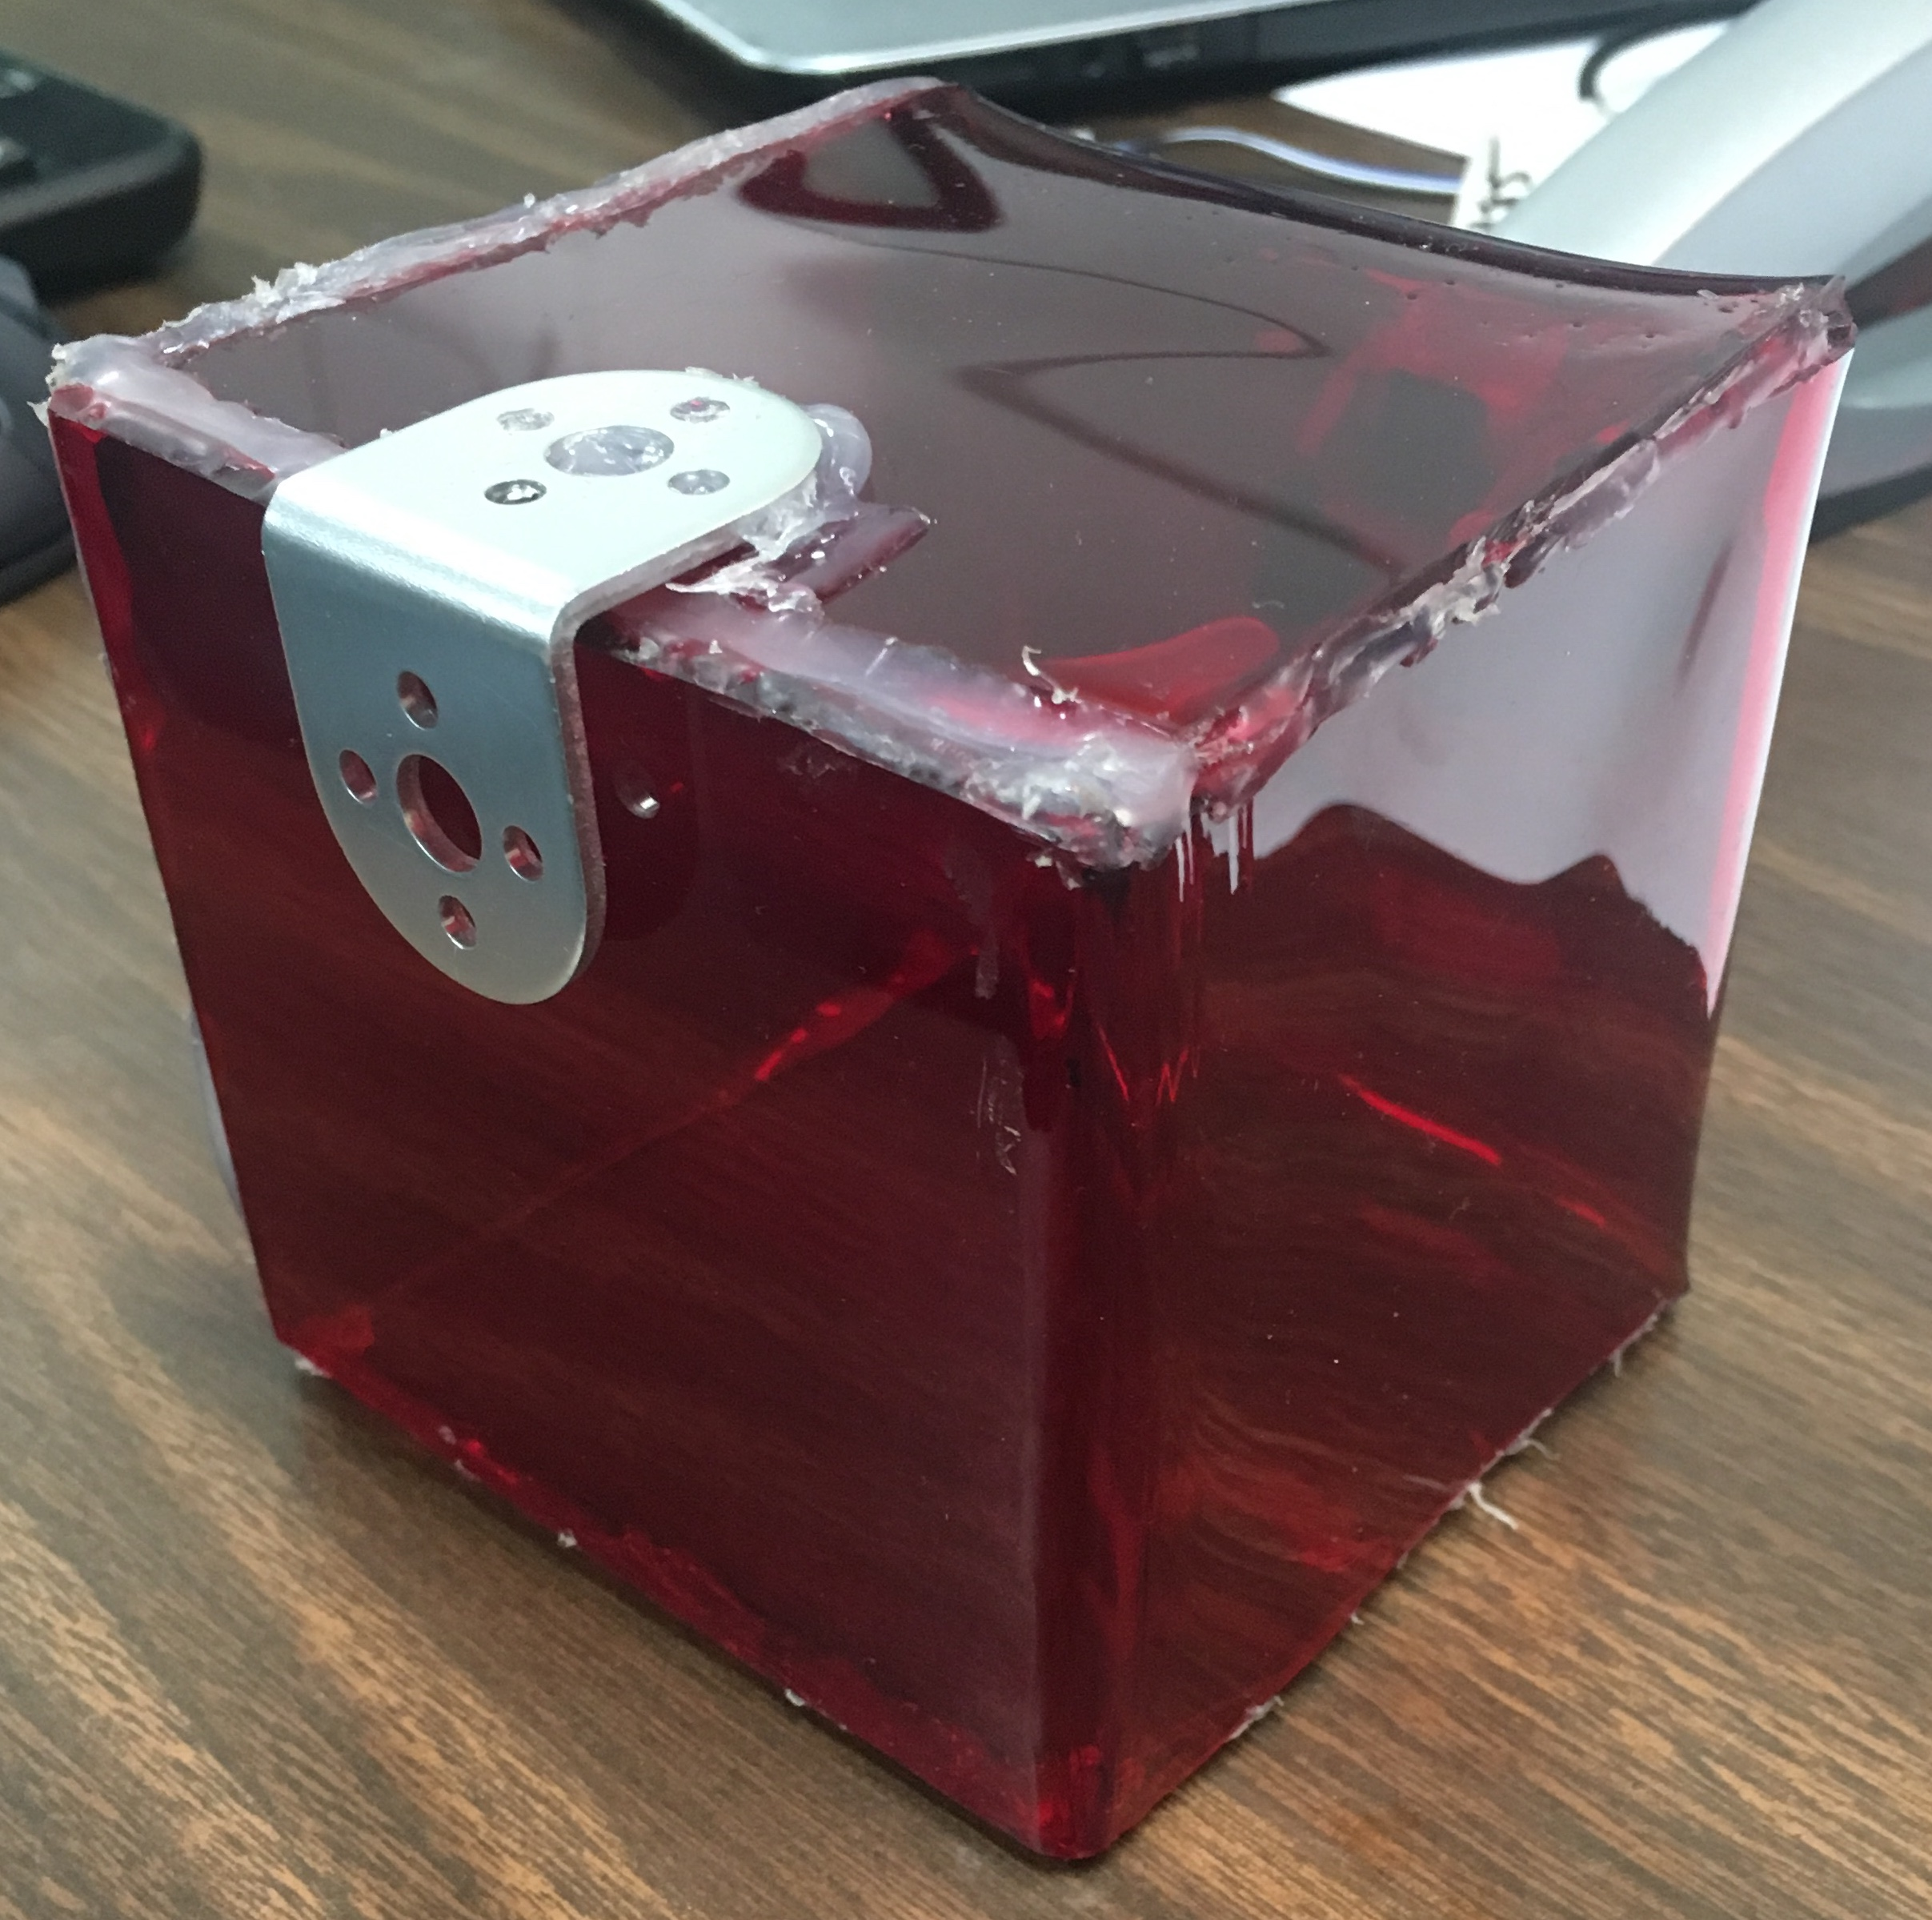
\includegraphics[width=.6\textwidth]{05_10-01/images/cube.jpg}
    \caption{Acrylic Cube}
    \label{fig:cube}
\end{figure}



\subsection{Drivetrain decision}
%! Decide on the design for the drivetrain.
The entire team made a matrix to help weight the pro and cons of the prototype drive-trains and already proven styles. The matrix took a lot in to consideration, such as agility, size, strength, traction, and maneuverability. The results of the matrix was a mecanum style drive-train driven by orbital 20 gearbox and belts. We choose this style because of its high speed, agility, and maneuverability, the downside to this style drive-train is the traction, which in turn can make playing defense a lot hard, compared to a none mecanum drive-train.  

\subsection{Develop custom lift}
%! Further investigate possible lift designs and weigh the pros and cons of each. 
The x-rail lift design would work, but Kelly still wanted to investigate the 254-style lift, with square tubing, bearings, and custom bearing blocks. While more labor-intensive and harder to pull off, the end result would be better than with x-rail if it turned out correctly. Where the x-rail only needed bearings on one side, because the v-bearings would be able to resolve both radial and lateral loads, normal bearings can only resolve radial loads, so bearings will have to be placed on at least three sides to constrain the lift in both dimensions. Since the lift is composed of two mirrored parts, connected by the frame of the first stage, Kelly could get away with only running bearings along three sides of each tube, excluding the outer one, because the bearings in the y-axis would push the two sides against each other, preventing the lift from shifting side-to-side. Each bearing assembly would consist of four bearings, two on either side of the tube pinching it, and two next to each other running along the inside of the tube. Kelly began the CAD by making 1 in by $\frac{1}{2}$ in by $\frac{1}{16}$ in wall aluminum tubing in 16 inch lengths. One of these would be mounted to the drivetrain, and the other would make up the vertical portion of the first stage, rolling along the fixed one. A bearing assembly would go at the top of the fixed one and the bottom of the moving one, keeping the bearings as far apart from each other as possible, distributing the load and stabilizing the lift. The inner carriage would be made out of a H-shaped arrangement of more tubes, with a bearing assembly mounted at the top and bottom of each side of the H. After considering mounting the bearings by sandwiching the tube between two machined plates, Kelly realized this would not support the inner bearings, so decided on machined blocks that would be fixed to the tube with rivets. The blocks would have a quarter inch hole on the side for attaching the pinching bearings, and hole at the top where a bolt would connect the two blocks and support the inner bearings. After assembling this, Kelly found there was not enough room on the vertical portion of the first stage for both sets of bearings to roll against it, so it was neccecary for them to be swapped out for one inch by one inch tubes instead. 

\end{document}
